% replace all text with your own text.
% in this template few examples are mention
\chapter{Methodology}
\label{ch:method} % Label for method chapter
Recognizing the need for early detection and management of cardiovascular conditions, we utilize machine learning algorithms to analyze patient data and predict the likelihood of heart disease. Our methodology encompasses data collection, preprocessing, feature extraction, model development, and evaluation, aiming to deliver a robust and effective predictive tool for doctors. By integrating innovative learning algorithms and conducting experiments, we aspire to contribute meaningful solutions and enhance patient outcomes in cardiovascular health.

\section{Algorithms Descriptions}
\subsection{Logistic Regression}
LR is a statistical method used for binary classification tasks. It models the probability of a binary outcome based on one or more predictor variables. In the context of heart disease prediction, LR can analyze patient parameters such as age, cholesterol levels, and blood pressure to estimate the likelihood of the presence of heart disease.

\subsection{Naïve Bayes}
NB is a probabilistic classifier based on Bayes' theorem with an assumption of independence between features. In heart disease prediction, Naïve Bayes can effectively analyze patient attributes and calculate the conditional probability of heart disease given the observed features. Its simplicity and computational efficiency make Naïve Bayes a popular choice for healthcare applications.

\subsection{Random Forest}
RF is an ensemble learning method that constructs a multitude of decision trees during training and outputs the mode of the classes (classification) or mean prediction (regression) of the individual trees. In heart disease prediction, Random Forest can analyze a large number of patient parameters and identify complex patterns associated with cardiovascular conditions.

\section{Implementations}
\subsection{Logistic Regression}
For LR implementation, we'll utilize the `LogisticRegression` class from the `sklearn.linear\_model` module. We'll preprocess the dataset, including handling missing values and scaling features, before fitting the model to the training data.
\subsection{Naïve Bayes}
For NB implementation, we'll use the `GaussianNB` class from the `sklearn.naive\_bayes` module. Similar to Logistic Regression, we'll preprocess the dataset and fit the model to the training data.
\subsection{Random Forest}
For RF implementation, we'll employ the `RandomForestClassifier` class from the `sklearn.ensemble` module. We'll preprocess the dataset and tune hyperparameters, such as the number of estimators and maximum depth, to optimize model performance.

\section{Experiments Design}
In our experimental approach to assess the predictive performance of each algorithm for heart disease, we'll begin by dividing our dataset into separate training and testing sets. This division ensures that the models are trained on a subset of the data and evaluated on an independent portion, enabling us to gauge their generalization capability. To further fortify the reliability of our findings, we'll employ cross-validation techniques. This involves iteratively partitioning the dataset into multiple subsets, training the models on different combinations, and validating them on the remaining data, thus providing a more comprehensive evaluation. Subsequently, we'll utilize a range of performance metrics, including accuracy, precision, recall, and F1-score, to quantify the algorithms' effectiveness. These metrics will allow us to discern not only the models' overall correctness but also their ability to precisely identify positive cases and recall them accurately. By meticulously analyzing these performance indicators, we aim to determine the most optimal approach for heart disease prediction, considering factors such as model interpretability and computational efficiency alongside predictive accuracy.

\section{Algorithms}
In our project, we implement three distinct machine learning algorithms—Logistic Regression, Random Forest, and Naive Bayes—to predict heart disease. Logistic Regression is a simple yet powerful algorithm used for binary classification tasks, where it models the probability of a binary outcome. Random Forest, on the other hand, is an ensemble learning method that constructs multiple decision trees and aggregates their predictions to improve accuracy. Naive Bayes is a probabilistic classifier based on Bayes' theorem, particularly effective for datasets with high dimensionality and strong feature independence assumptions. Each algorithm offers unique advantages and approaches in identifying patterns and making predictions, contributing to our comprehensive analysis of heart disease prediction.

\begin{algorithm}
    \caption{Logistic Regression}
    \label{algo:logistic_regression}
    \begin{algorithmic}[1]
        \Require{Training dataset $(X_{train}, Y_{train})$, Test dataset $X_{test}$}
        \Ensure{Predicted class labels for $X_{test}$}
        \Statex
        \Function{LogisticRegression}{$X_{train}, Y_{train}, X_{test}$}
        \State Initialize logistic regression classifier
        \State Standardize features: $X_{train} \gets \text{StandardScaler.fit\_transform}(X_{train})$
        \State Fit classifier to training data: $classifier.fit(X_{train}, Y_{train})$
        \State Standardize test features: $X_{test} \gets \text{StandardScaler.transform}(X_{test})$
        \State Predict probabilities for test data: $y_{prob} \gets classifier.predict\_proba(X_{test})$
        \State Convert probabilities to class labels: $y_{pred} \gets \text{threshold\_function}(y_{prob})$
        \State \Return $y_{pred}$
        \EndFunction
    \end{algorithmic}
\end{algorithm}

\begin{algorithm}
    \caption{Random Forest}
    \label{algo:random_forest}
    \begin{algorithmic}[1]
        \Require{Training dataset $(X_{train}, Y_{train})$, Test dataset $X_{test}$}
        \Ensure{Predicted class labels for $X_{test}$}
        \Statex
        \Function{RandomForest}{$X_{train}, Y_{train}, X_{test}$}
        \State Initialize random forest classifier with specified parameters
        \State Handle missing values: $X_{train}, X_{test} \gets \text{Imputer.fit\_transform}(X_{train}, X_{test})$
        \State Fit classifier to training data: $classifier.fit(X_{train}, Y_{train})$
        \State Predict class labels for test data: $y_{pred} \gets classifier.predict(X_{test})$
        \State \Return $y_{pred}$
        \EndFunction
    \end{algorithmic}
\end{algorithm}

\begin{algorithm}
    \caption{Naive Bayes}
    \label{algo:naive_bayes}
    \begin{algorithmic}[1]
        \Require{Training dataset $(X_{train}, Y_{train})$, Test dataset $X_{test}$}
        \Ensure{Predicted class labels for $X_{test}$}
        \Statex
        \Function{NaiveBayes}{$X_{train}, Y_{train}, X_{test}$}
        \State Initialize naive Bayes classifier
        \State Discretize continuous features: $X_{train}, X_{test} \gets \text{Binarizer.fit\_transform}(X_{train}, X_{test})$
        \State Fit classifier to training data: $classifier.fit(X_{train}, Y_{train})$
        \State Predict class labels for test data: $y_{pred} \gets classifier.predict(X_{test})$
        \State \Return $y_{pred}$
        \EndFunction
    \end{algorithmic}
\end{algorithm}


\begin{figure}
    \centering
    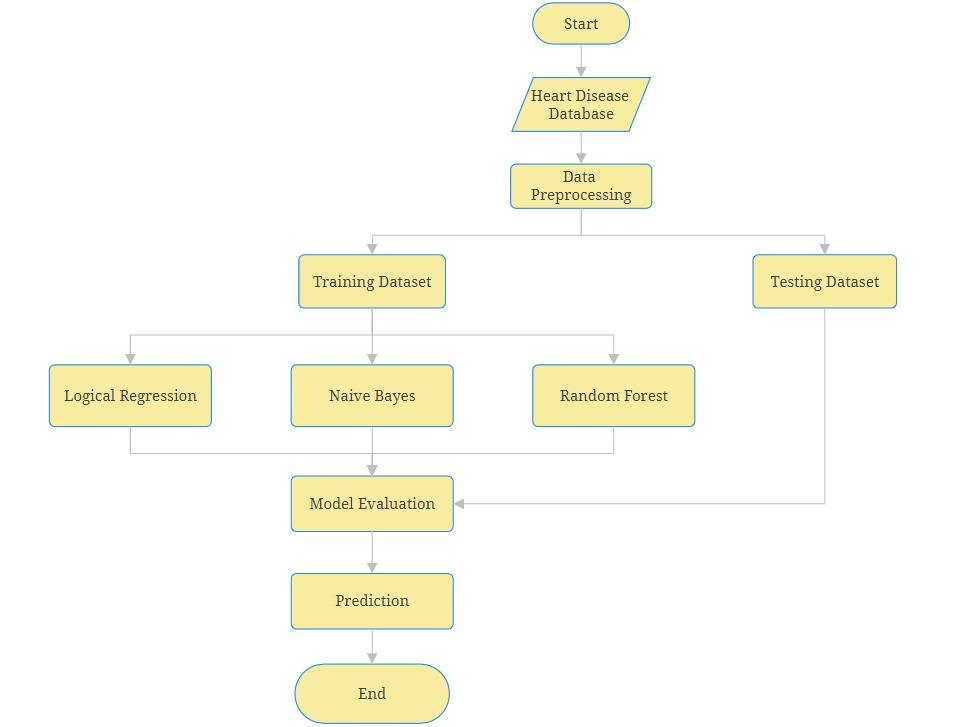
\includegraphics[width=1\linewidth]{figures/Flowchart.jpg}
    \caption{Flowchart of Heart Disease Prediction using LR, RF and NB}
    \label{fig:enter-label}
\end{figure}


\section{Code}
\subsection{Data Pre-processing}
\begin{lstlisting}[language=Python, label=list:python_code_ex]
# Importing the libraries

import numpy as np
import matplotlib.pyplot as plt
import pandas as pd

from sklearn.impute import SimpleImputer
from sklearn.model_selection import train_test_split
from sklearn.preprocessing import StandardScaler
from sklearn.metrics import accuracy_score
from sklearn.metrics import confusion_matrix
from sklearn.metrics import classification_report
from sklearn.metrics import roc_auc_score
from sklearn.metrics import roc_curve

# Importing the dataset
dataset = pd.read_csv('cleve.csv')

#defining X values ang y values
X = dataset.iloc[:, :-1].values
Y = dataset.iloc[:, 13].values

#handling missing data
imputer= SimpleImputer(missing_values=np.nan, strategy='mean')
imputer=imputer.fit(X[:,11:13])
X[:,11:13]=imputer.transform(X[:,11:13])

#splitting dataset into training set and test set
X_train,X_test,Y_train,Y_test=train_test_split(X, Y, test_size = 0.25, random_state = 101)

#feature scaling
s=StandardScaler()
X_train=s.fit_transform(X_train)
X_test=s.transform(X_test)
\end{lstlisting}

\clearpage  %

\subsection{Logistic Regression}
\begin{lstlisting}[language=Python, label=list:python_code_ex]
#fitting LR to training set
from sklearn.linear_model import LogisticRegression
LogisticRegressionClassifier =LogisticRegression()
LogisticRegressionClassifier.fit(X_train,Y_train)

#Predict the test set results
Y_pred=LogisticRegressionClassifier.predict(X_test)

#checking the accuracy for predicted results
accuracy_score(Y_test,Y_pred)

# Making the Confusion Matrix
cm = confusion_matrix(Y_test, Y_pred)

#Interpretation:
print(classification_report(Y_test, Y_pred))
\end{lstlisting}

\begin{table}[h!]
    \centering
    \caption{Classification Report of LR}
    \label{tab:_ex_tab}
    \begin{tabular}{ccccc}     
        \toprule
            &  precision & recall & f1-score & support \\
        \midrule
        0 & 0.81 & 0.94 & 0.87 & 36 \\
        1 & 0.94 & 0.80 & 0.86 & 40 \\

        accuracy & - & - & 0.87 & 76 \\
        macro avg & 0.88 & 0.87 & 0.87 & 76 \\
        weighted avg & 0.88 & 0.87 & 0.87 & 76 \\
        \bottomrule
    \end{tabular}
\end{table}

\begin{lstlisting}[language=Python, label=list:python_code_ex]
#ROC
logit_roc_auc = roc_auc_score(Y_test, LogisticRegressionClassifier.predict(X_test))
fpr, tpr, thresholds = roc_curve(Y_test, LogisticRegressionClassifier.predict_proba(X_test)[:,1])
plt.figure()
plt.plot(fpr, tpr, label='Logistic Regression (area = %0.2f)' % logit_roc_auc)
plt.plot([0, 1], [0, 1],'r--')
plt.xlim([0.0, 1.0])
plt.ylim([0.0, 1.05])
plt.xlabel('False Positive Rate')
plt.ylabel('True Positive Rate')
plt.title('Receiver operating characteristic')
plt.legend(loc="lower right")
plt.savefig('Log_ROC')
plt.show()

#PREDICTION FOR NEW DATASET using LogisticRegressionClassifier
Newdataset = pd.read_csv('newdata.csv')
ynew=LogisticRegressionClassifier.predict(Newdataset)
print("Predicted Class for newdata.csv:",ynew)
\end{lstlisting}

\begin{figure}
    \centering
    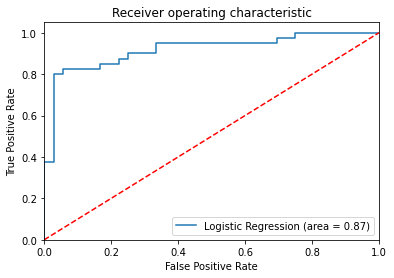
\includegraphics[width=0.5\linewidth]{LR.png}
    \caption{Receiver operating characteristics of LR}
    \label{fig:enter-label}
\end{figure}

\subsection{Random Forest}
\begin{lstlisting}[language=Python, label=list:python_code_ex]
# Fitting RandomForestClassifier to the Training set
from sklearn.ensemble import RandomForestClassifier
RandomForestClassifier =RandomForestClassifier(n_estimators=20)
RandomForestClassifier.fit(X_train, Y_train)

# Predicting the Test set results
Y_pred2 = RandomForestClassifier.predict(X_test)
from sklearn.metrics import accuracy_score
accuracy_score(Y_test,Y_pred2)

# Making the Confusion Matrix
from sklearn.metrics import confusion_matrix
cm = confusion_matrix(Y_test, Y_pred2)

#Interpretation:
print(classification_report(Y_test, Y_pred2))
\end{lstlisting}

\begin{table}[h!]
    \centering
    \caption{Classification Report of RF}
    \label{tab:_ex_tab}
    \begin{tabular}{ccccc}     
        \toprule
            &  precision & recall & f1-score & support \\
        \midrule
        0 & 0.80 & 0.89 & 0.84 & 36 \\
        1 & 0.89 & 0.80 & 0.84 & 40 \\

        accuracy & - & - & 0.84 & 76 \\
        macro avg & 0.84 & 0.84 & 0.84 & 76 \\
        weighted avg & 0.85 & 0.84 & 0.84 & 76 \\
        \bottomrule
    \end{tabular}
\end{table}

\clearpage  %

\begin{lstlisting}[language=Python, label=list:python_code_ex]
#ROC
from sklearn.metrics import roc_auc_score
from sklearn.metrics import roc_curve
logit_roc_auc = roc_auc_score(Y_test, RandomForestClassifier.predict(X_test))
fpr, tpr, thresholds = roc_curve(Y_test, RandomForestClassifier.predict_proba(X_test)[:,1])
plt.figure()
plt.plot(fpr, tpr, label='Random Forest (area = %0.2f)' % logit_roc_auc)
plt.plot([0, 1], [0, 1],'r--')
plt.xlim([0.0, 1.0])
plt.ylim([0.0, 1.05])
plt.xlabel('False Positive Rate')
plt.ylabel('True Positive Rate')
plt.title('Receiver operating characteristic')
plt.legend(loc="lower right")
plt.savefig('RF_ROC')
plt.show()

#PREDICTION FOR NEW DATASET using RandomForest
ynew=RandomForestClassifier.predict(Newdataset)
print("Predicted Class for newdata.csv:",ynew)
\end{lstlisting}

\begin{figure}[H]
    \centering
    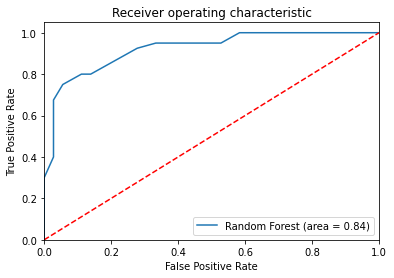
\includegraphics[width=0.5\linewidth]{RF.png}
    \caption{Receiver operating characteristics of RF}
    \label{fig:enter-label}
\end{figure}

\subsection{Naive Bayes}
\begin{lstlisting}[language=Python, label=list:python_code_ex]
NaiveBayesimputer= SimpleImputer(strategy='mean')
NaiveBayesimputer=NaiveBayesimputer.fit(X[:,11:13])
X[:,11:13]=NaiveBayesimputer.transform(X[:,11:13])

#splitting dataset into training set and test set
X_train,X_test,Y_train,Y_test=train_test_split(X, Y, test_size = 0.25, random_state = None)

# Fitting Naive Bayes to the Training set
from sklearn.naive_bayes import GaussianNB
NaiveBayesClassifier = GaussianNB()
NaiveBayesClassifier.fit(X_train, Y_train)


# Predicting the Test set results
Y_pred3 = NaiveBayesClassifier.predict(X_test)
#ACCURACY SCORE
accuracy_score(Y_test,Y_pred3)

# Making the Confusion Matrix
cm = confusion_matrix(Y_test, Y_pred3)

#Interpretation:
print(classification_report(Y_test, Y_pred3))
\end{lstlisting}

\begin{table}[h!]
    \centering
    \caption{Classification Report of NB}
    \label{tab:_ex_tab}
    \begin{tabular}{ccccc}     
        \toprule
            &  precision & recall & f1-score & support \\
        \midrule
        0 & 0.80 & 0.90 & 0.84 & 39 \\
        1 & 0.88 & 0.76 & 0.81 & 37 \\

        accuracy & - & - & 0.83 & 76 \\
        macro avg & 0.84 & 0.83 & 0.83 & 76 \\
        weighted avg & 0.83 & 0.83 & 0.83 & 76 \\
        \bottomrule
    \end{tabular}
\end{table}


\begin{lstlisting}[language=Python, label=list:python_code_ex]
#ROC
logit_roc_auc = roc_auc_score(Y_test,NaiveBayesClassifier.predict(X_test))
fpr, tpr, thresholds = roc_curve(Y_test, NaiveBayesClassifier.predict_proba(X_test)[:,1])
plt.figure()
plt.plot(fpr, tpr, label='Navie Bayes (area = %0.2f)' % logit_roc_auc)
plt.plot([0, 1], [0, 1],'r--')
plt.xlim([0.0, 1.0])
plt.ylim([0.0, 1.05])
plt.title('Receiver operating characteristic')
plt.legend(loc="lower right")
plt.savefig('NB_ROC')
plt.show()

#PREDICTION FOR NEW DATASET using NaiveBayesClassifier
ynew = NaiveBayesClassifier.predict(Newdataset)
print("Predicted Class for newdata.csv:", ynew)
\end{lstlisting}

\begin{figure}[H]
    \centering
    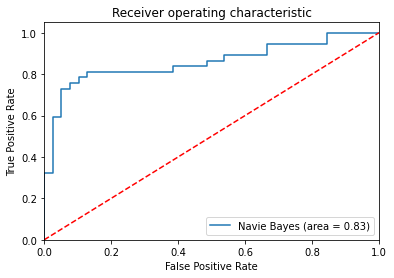
\includegraphics[width=0.4\linewidth]{NB.png}
    \caption{Receiver operating characteristics of NB}
    \label{fig:enter-label}
\end{figure}